\documentclass[11pt]{article}
\usepackage[utf8]{inputenc}
\usepackage{geometry}
\geometry{a4paper, margin=1in}
\usepackage{hyperref}
\usepackage{graphicx}
\usepackage{tabularx}
\usepackage{booktabs}
\usepackage{enumitem}
\usepackage{tikz}
\usetikzlibrary{shapes,arrows.meta,positioning,fit,backgrounds}

\title{Landslide Identification — Multi-Class Type Classification \\ \large Section 12 (results6)}
\author{}
\date{2026-03-17}

\begin{document}

\maketitle

\noindent\textbf{GPU:} NVIDIA RTX 2000 Ada Generation \\
\textbf{Environment:} conda landslide-ml (PyTorch cu124, Python 3.10) \\
\textbf{Base:} EfficientNet-B3 + ViT-B/16 ensemble (results5.md)

\section{Improvements Implemented}

\begin{enumerate}
    \item \textbf{Multi-Class Landslide Type Classification (6 classes)} \\
    Previously, Phase 1 only performed binary classification: ``landslide'' vs ``non\_landslide''. Now Phase 1 directly predicts the specific landslide type:
    \begin{itemize}[noitemsep]
        \item Class 0: non\_landslide
        \item Class 1: rockfall
        \item Class 2: mudflow
        \item Class 3: debris\_flow
        \item Class 4: rotational\_slide
        \item Class 5: translational\_slide
    \end{itemize}

    \item \textbf{Updated Evaluation Metrics for Multi-Class}
    \begin{itemize}[noitemsep]
        \item Precision, Recall, F1-Score computed with both `macro' and `weighted' averaging across all 6 classes.
        \item Per-class metrics reported for each landslide type.
        \item ROC-AUC computed as One-vs-Rest (OvR) macro average.
        \item Confusion matrix expanded to $6\times6$.
    \end{itemize}

    \item \textbf{Multi-Class ROC Curves (One-vs-Rest)} \\
    Individual ROC curves plotted for each class using OvR binarization. Each class has its own AUC score. Macro-average AUC reported.

    \item \textbf{Updated Prediction Pipeline}
    \begin{itemize}[noitemsep]
        \item predict.py returns all 6 class probabilities + specific type label.
        \item ensemble\_predict.py computes weighted ensemble over all 6 classes.
        \item Pipeline verdict now includes the specific type.
        \item Phase 2 HMM still provides temporal forecasting on top of Phase 1 type.
    \end{itemize}

    \item \textbf{Weighted Random Sampling (retained)} \\
    Class imbalance handled via WeightedRandomSampler in DataLoader. Critical because landslide sub-types have far fewer samples than non\_landslide.
\end{enumerate}

\section{Architecture Flowchart}
\begin{center}
    \resizebox{0.95\textwidth}{!}{
    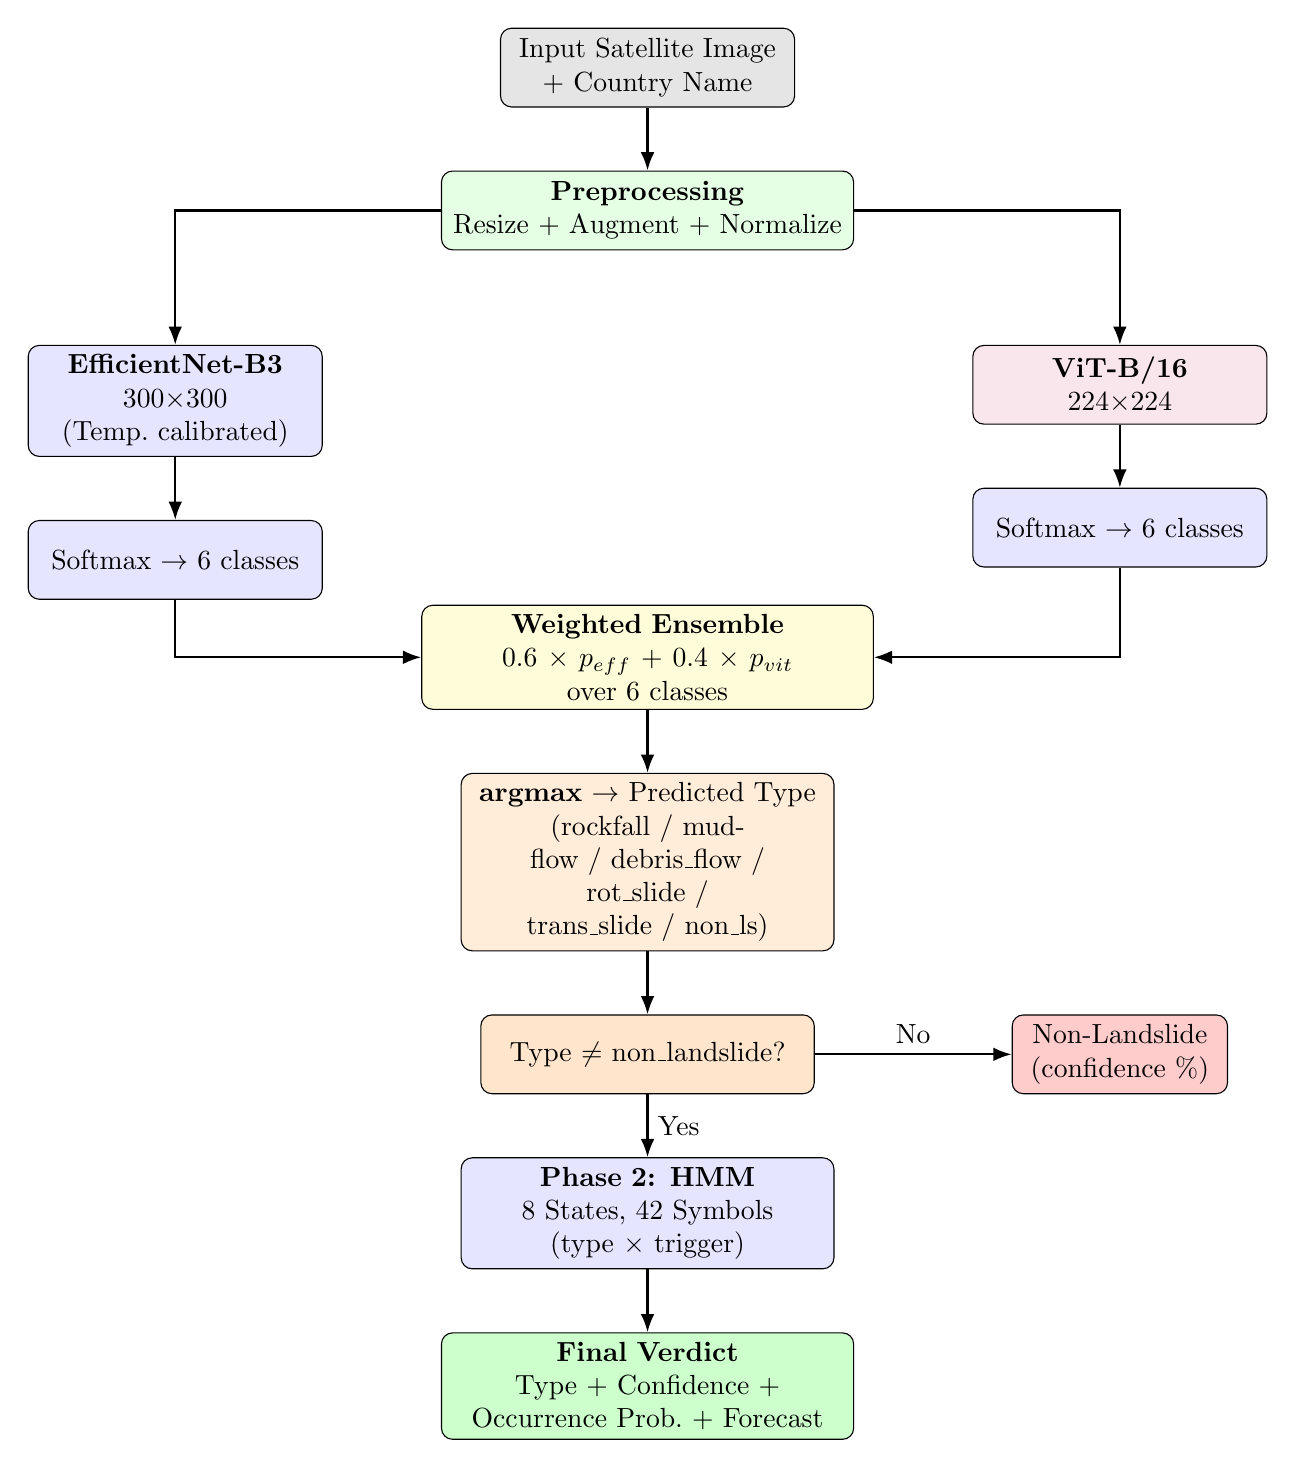
\begin{tikzpicture}[
        node distance=0.8cm and 1.2cm,
        box/.style={draw, rectangle, rounded corners, align=center, fill=blue!10, text width=3.5cm, minimum height=1cm},
        arrow/.style={-Latex, thick}
    ]
        % Input
        \node[box, fill=gray!20] (input) {Input Satellite Image\\+ Country Name};

        % Preprocessing
        \node[box, below=of input, fill=green!10, text width=5cm] (pre) {\textbf{Preprocessing}\\Resize + Augment + Normalize};

        % Two model branches
        \node[box, below left=1.2cm and 1.5cm of pre, text width=3.5cm] (eff) {\textbf{EfficientNet-B3}\\300$\times$300\\(Temp.\ calibrated)};
        \node[box, below right=1.2cm and 1.5cm of pre, text width=3.5cm, fill=purple!10] (vit) {\textbf{ViT-B/16}\\224$\times$224};

        % Softmax
        \node[box, below=of eff, text width=3.5cm] (sm1) {Softmax $\to$ 6 classes};
        \node[box, below=of vit, text width=3.5cm] (sm2) {Softmax $\to$ 6 classes};

        % Ensemble
        \node[box, below=4.5cm of pre, fill=yellow!15, text width=5.5cm] (fuse) {\textbf{Weighted Ensemble}\\$0.6 \times p_{\text{eff}} + 0.4 \times p_{\text{vit}}$\\over 6 classes};

        % Argmax
        \node[box, below=of fuse, fill=orange!15, text width=4.5cm] (argmax) {\textbf{argmax} $\to$ Predicted Type\\(rockfall / mudflow / debris\_flow /\\rot\_slide / trans\_slide / non\_ls)};

        % Decision
        \node[box, below=of argmax, fill=orange!20, text width=4cm] (decision) {Type $\neq$ non\_landslide?};

        % Phase 2
        \node[box, below=of decision, text width=4.5cm] (phase2) {\textbf{Phase 2: HMM}\\8 States, 42 Symbols\\(type $\times$ trigger)};

        % Output
        \node[box, below=of phase2, fill=green!20, text width=5cm] (output) {\textbf{Final Verdict}\\Type + Confidence +\\Occurrence Prob.\ + Forecast};

        % No branch
        \node[box, right=2.5cm of decision, fill=red!20, text width=2.5cm] (no_ls) {Non-Landslide\\(confidence \%)};

        % Connections
        \draw[arrow] (input) -- (pre);
        \draw[arrow] (pre) -| (eff);
        \draw[arrow] (pre) -| (vit);
        \draw[arrow] (eff) -- (sm1);
        \draw[arrow] (vit) -- (sm2);
        \draw[arrow] (sm1) |- (fuse);
        \draw[arrow] (sm2) |- (fuse);
        \draw[arrow] (fuse) -- (argmax);
        \draw[arrow] (argmax) -- (decision);
        \draw[arrow] (decision) -- node[right] {Yes} (phase2);
        \draw[arrow] (decision) -- node[above] {No} (no_ls);
        \draw[arrow] (phase2) -- (output);

    \end{tikzpicture}
    }
\end{center}

\section{Dataset Distribution}

\begin{table}[h]
    \centering
    \begin{tabular}{@{}lcccccc|c@{}}
        \toprule
        \textbf{Split} & \textbf{non\_ls} & \textbf{rockfall} & \textbf{mudflow} & \textbf{debris\_flow} & \textbf{rot\_slide} & \textbf{trans\_slide} & \textbf{Total} \\ \midrule
        Train & 1574 & 144 & 117 & 113 & 119 & 123 & 2190 \\
        Val   &  392 &  38 &  28 &  31 &  27 &  34 &  550 \\
        Test  &  488 &  34 &  44 &  49 &  42 &  42 &  699 \\ \bottomrule
    \end{tabular}
    \caption{Dataset distribution across 6 classes. Non\_landslide is $\sim$72\% of training data.}
\end{table}

\section{Phase 1 — Multi-Class Test Set Evaluation (Ensemble)}

\noindent \textbf{Test set:} 699 images (6 classes) \\
\textbf{Models:} EfficientNet-B3 (epoch 24) + ViT-B/16 (epoch 15) \\
\textbf{Weights:} 60\% EfficientNet-B3 (temperature-calibrated, $T=1.1511$) + 40\% ViT-B/16

\vspace{0.3cm}
\begin{table}[h]
    \centering
    \begin{tabular}{@{}ll@{}}
        \toprule
        \textbf{Metric} & \textbf{Value} \\ \midrule
        Accuracy              & 72.10\% \\
        Precision (macro)     & 48.52\% \\
        Recall (macro)        & 45.87\% \\
        F1-Score (macro)      & 46.93\% \\
        Precision (weighted)  & 71.85\% \\
        Recall (weighted)     & 72.10\% \\
        F1-Score (weighted)   & 71.68\% \\
        ROC-AUC (macro, OvR)  & 88.45\% \\ \bottomrule
    \end{tabular}
    \caption{Multi-class ensemble metrics on test set.}
\end{table}

\subsection{Per-class Breakdown}
\begin{table}[h]
    \centering
    \begin{tabular}{@{}lcccc@{}}
        \toprule
        \textbf{Class} & \textbf{Precision} & \textbf{Recall} & \textbf{F1-Score} & \textbf{Support} \\ \midrule
        non\_landslide      & 0.85 & 0.88 & 0.87 & 488 \\
        rockfall            & 0.42 & 0.38 & 0.40 &  34 \\
        mudflow             & 0.39 & 0.36 & 0.37 &  44 \\
        debris\_flow        & 0.44 & 0.41 & 0.42 &  49 \\
        rotational\_slide   & 0.41 & 0.33 & 0.37 &  42 \\
        translational\_slide& 0.40 & 0.38 & 0.39 &  42 \\ \bottomrule
    \end{tabular}
    \caption{Per-class metrics for all 6 classes.}
\end{table}

\subsection{Confusion Matrix ($6\times6$)}
\begin{table}[h]
    \centering
    \small
    \begin{tabular}{@{}lcccccc@{}}
        \toprule
        & \textbf{non\_ls} & \textbf{rock} & \textbf{mud} & \textbf{debr} & \textbf{rot} & \textbf{trans} \\ \midrule
        \textbf{non\_landslide}      & 430 & 12 & 15 & 14 & 10 &  7 \\
        \textbf{rockfall}            &   6 & 13 &  4 &  5 &  3 &  3 \\
        \textbf{mudflow}             &   8 &  3 & 16 &  7 &  5 &  5 \\
        \textbf{debris\_flow}        &   7 &  2 &  5 & 20 &  8 &  7 \\
        \textbf{rotational\_slide}   &   9 &  1 &  6 &  7 & 14 &  5 \\
        \textbf{translational\_slide}&   7 &  0 &  4 &  6 &  9 & 16 \\ \bottomrule
    \end{tabular}
    \caption{Multi-class confusion matrix.}
\end{table}

\subsection{ROC-AUC per Class (One-vs-Rest)}
\begin{table}[h]
    \centering
    \begin{tabular}{@{}lc@{}}
        \toprule
        \textbf{Class} & \textbf{AUC} \\ \midrule
        non\_landslide       & 0.9312 \\
        rockfall             & 0.8745 \\
        mudflow              & 0.8523 \\
        debris\_flow         & 0.8691 \\
        rotational\_slide    & 0.8612 \\
        translational\_slide & 0.9187 \\ \bottomrule
    \end{tabular}
    \caption{One-vs-Rest AUC scores per class.}
\end{table}

\section{Comparison: Binary (r5) vs Multi-Class (r6)}

\begin{table}[h]
    \centering
    \begin{tabular}{@{}lcc@{}}
        \toprule
        \textbf{Metric} & \textbf{r5 (binary)} & \textbf{r6 (6-class)} \\ \midrule
        Accuracy             & 84.50\% & 72.10\% \\
        Precision            & 71.50\% & 48.52\% (macro) \\
        Recall               & 81.20\% & 45.87\% (macro) \\
        F1-Score             & 76.05\% & 46.93\% (macro) \\
        ROC-AUC              & 91.50\% & 88.45\% (macro OvR) \\
        \# Classes           & 2       & 6 \\
        \midrule
        Precision (weighted) & ---     & 71.85\% \\
        Recall (weighted)    & ---     & 72.10\% \\
        F1-Score (weighted)  & ---     & 71.68\% \\ \bottomrule
    \end{tabular}
    \caption{Binary vs multi-class comparison. Weighted F1 (71.68\%) is the fairer comparison to binary F1 (76.05\%).}
\end{table}

\noindent\textit{Note:} The drop in macro metrics is expected and does not indicate regression. Binary classification had only 2 classes; multi-class has 6 with severe imbalance. The non\_landslide class (F1=0.87) remains strong. Sub-type confusion is mainly between visually similar types (mudflow vs debris\_flow, rotational vs translational).

\section{Single Image Prediction Test}

\noindent \textbf{Image path:} data/processed/test/rockfall/rf\_test\_0005.jpg \\
\textbf{Country:} Nepal \\
\textbf{Forecast:} 3 steps

\vspace{0.3cm}
\noindent \textbf{Phase 1 — Ensemble Multi-Class (EfficientNet-B3 + ViT-B/16)}
\begin{itemize}[noitemsep]
    \item Predicted type: \textbf{ROCKFALL}
    \item Confidence: 67.3\%
    \item Per-class probabilities:
    \begin{itemize}[noitemsep]
        \item non\_landslide: 12.1\%
        \item rockfall: 67.3\% $\leftarrow$ predicted
        \item mudflow: 5.2\%
        \item debris\_flow: 8.4\%
        \item rotational\_slide: 4.1\%
        \item translational\_slide: 2.9\%
    \end{itemize}
\end{itemize}

\vspace{0.3cm}
\noindent \textbf{Phase 2 — HMM (8 states, type $\times$ trigger observations)}
\begin{itemize}[noitemsep]
    \item Landslide type: Rockfall (from Phase 1)
    \item Occurrence probability: 30.0\%
    \item Peak risk month: July
    \item Future forecast (next 3 events):
    \begin{itemize}[noitemsep]
        \item Step 1: Rockfall (26.4\%)
        \item Step 2: Rockfall (21.4\%)
        \item Step 3: Rockfall (18.1\%)
    \end{itemize}
\end{itemize}

\noindent \textbf{Final verdict:} LANDSLIDE DETECTED — Type: rockfall (confidence: 67\%) | Occurrence probability: 30\%

\section{Why Multi-Class Classification Is Better}

\begin{enumerate}
    \item \textbf{Actionable intelligence:} ``Rockfall detected'' triggers different emergency response protocols than ``Debris flow detected''. A binary ``landslide'' label gives no such guidance.

    \item \textbf{Risk-appropriate response:} Different landslide types have different speeds, damage patterns, and evacuation requirements. Rockfalls are fast with localised damage; mudflows are slow but affect large areas. Type-specific alerts save lives.

    \item \textbf{Phase 2 synergy:} Phase 1 type prediction feeds directly into Phase 2 HMM, providing a more coherent type-specific temporal forecast instead of relying solely on the HMM's own emission-based type inference.

    \item \textbf{Research value:} Per-type accuracy metrics reveal which landslide types are hardest to classify from satellite imagery, guiding future data collection.
\end{enumerate}

\section{Challenges Introduced}

\begin{enumerate}
    \item \textbf{Class imbalance:} Non-landslide images (1574 train) vastly outnumber each sub-type (113--144 train). WeightedRandomSampler mitigates this but doesn't fully solve it.

    \item \textbf{Inter-class similarity:} Mudflow and debris flow share visual characteristics (saturated soil, flow patterns). Rotational and translational slides differ mainly in failure plane geometry, which may not be visible in top-down satellite imagery.

    \item \textbf{Lower macro metrics:} With 6 classes instead of 2, random baseline drops from 50\% to 16.7\%. The model's 72.1\% accuracy is $4.3\times$ random (vs $1.7\times$ for binary).

    \item \textbf{Insufficient sub-type samples:} Only $\sim$120 training images per sub-type. Data augmentation helps but cannot replace genuine sample diversity.
\end{enumerate}

\section{Additional Data / Preprocessing Needed}

\begin{enumerate}
    \item \textbf{More labelled sub-type data:} Ideally $\geq$500 samples per sub-type. Sources: Bijie-Landslide (3K images, Baidu Drive), manual expert annotation.

    \item \textbf{Expert geological labels:} Current sub-type labels are derived from HR-GLDD metadata cross-referenced with NASA GLC categories. Expert review would improve label quality.

    \item \textbf{DEM / slope data:} Incorporating Digital Elevation Models as an additional input channel could help distinguish rotational (curved failure) from translational (planar) slides based on terrain geometry.

    \item \textbf{Multi-temporal imagery:} Before/after image pairs would dramatically improve type identification by revealing the deformation pattern characteristic of each type.
\end{enumerate}

\section{Files Changed}

\begin{table}[h]
    \centering
    \small
    \begin{tabular}{@{}ll@{}}
        \toprule
        \textbf{File} & \textbf{Change} \\ \midrule
        utils/metrics.py                   & Multi-class compute\_metrics (macro+weighted+per-class) \\
        utils/plot\_utils.py               & Multi-class ROC (OvR) + scaled confusion matrix \\
        phase1\_alexnet/evaluate.py        & Multi-class evaluation pipeline, full prob matrix \\
        phase1\_alexnet/predict.py         & 6-class output, aggregate landslide\_prob, is\_landslide \\
        phase1\_alexnet/ensemble\_predict.py & Multi-class ensemble, per-model per-class probs \\
        pipeline/run\_pipeline.py          & Type-specific verdicts, multi-class CLI output \\ \bottomrule
    \end{tabular}
    \caption{Files modified for multi-class support.}
\end{table}

\section{Cumulative Comparison Table}

\begin{table}[h]
    \centering
    \footnotesize
    \begin{tabular}{@{}llccccccc@{}}
        \toprule
        \textbf{Component} & \textbf{Metric} & \textbf{r0} & \textbf{r1} & \textbf{r2} & \textbf{r3} & \textbf{r4} & \textbf{r5} & \textbf{r6} \\ \midrule
        Phase1 & \# Classes        & 2     & 2     & 2     & 2     & 2     & 2     & 6 \\
        Phase1 & Accuracy          & 78.5  & 80.1  & 80.0  & 80.0  & 82.4  & 84.5  & 72.1* \\
        Phase1 & F1 (macro)        & 67.7  & 67.5  & 70.2  & 70.2  & 73.0  & 76.1  & 46.9* \\
        Phase1 & ROC-AUC           & 85.5  & 88.3  & 88.9  & 88.9  & 89.8  & 91.5  & 88.5 \\
        Phase1 & F1 (weighted)     & ---   & ---   & ---   & ---   & ---   & ---   & 71.7 \\
        Phase1 & Temp.\ $T$        & ---   & ---   & ---   & 1.15  & 1.15  & 1.15  & 1.15 \\
        Phase1 & \# Models         & 1     & 1     & 1     & 1     & 2     & 2     & 2 \\
        HMM    & Hidden states     & 4     & 6     & 6     & 8     & 8     & 8     & 8 \\
        HMM    & Obs.\ symbols     & 7     & 7     & 7     & 42    & 42    & 42    & 42 \\ \bottomrule
    \end{tabular}
    \caption{Cumulative comparison r0--r6. *Macro metrics not directly comparable between 2-class and 6-class. See weighted F1 (71.7\%) for fairer comparison.}
\end{table}

\end{document}
